\documentclass[11pt,a4paper]{article}
\usepackage[utf8]{inputenc}
\usepackage[T1]{fontenc}
\usepackage[margin=1in,top=1.2in,bottom=1.2in]{geometry}
\usepackage{microtype}
\usepackage{graphicx}
\usepackage{hyperref}
\usepackage{enumitem}
\usepackage{amsmath}
\usepackage{amsfonts}
\usepackage{amssymb}
\usepackage{longtable}
\usepackage{booktabs}
\usepackage{xcolor}
\usepackage{parskip}
\usepackage{float}
\usepackage{tikz}
\usetikzlibrary{positioning, arrows.meta}

% Better line breaking
\sloppy
\emergencystretch=3em
\hyphenpenalty=1000
\tolerance=1000

% Title formatting - handle long titles
\makeatletter
\renewcommand{\@maketitle}{
  \begin{center}
  {\Large \bfseries \begin{minipage}{0.9\textwidth} \centering \@title \end{minipage} \par}
  \vspace{1em}
  {\large \@author \par}
  \vspace{0.5em}
  {\normalsize \@date \par}
  \end{center}
  \vspace{1em}
}
\makeatother

\title{A System and Method for Spatiotemporal Object Detection Using Hybrid Single-Photon Time-of-Flight and Active Pixel Sensors}
\author{A. Akuoko, D. Chitnis, and I. Gyongy}
\date{\today}

\begin{document}
\maketitle
\newpage

\subsection{ABSTRACT}

A system and method for enhanced object detection and material classification through the fusion of spatially resolved intensity images and time-resolved transient signals. The system comprises a single-photon avalanche diode (SPAD) time-of-flight sensor configured to capture one-dimensional temporal photon arrival histograms, an active pixel sensor (APS) configured to capture two-dimensional spatially resolved RGB intensity images, and a dual-model processing architecture. The spatial detection module processes RGB images for object localisation and classification, while the material detection module processes transient signals for material composition classification. The system achieves combined detection performance of 94.5% to 98.5% accuracy with near-real-time processing speeds of approximately 8 milliseconds, enabling reliable material-aware scene understanding for safety-critical applications including autonomous vehicles and robotic manipulation.

\vspace{0.5em}
\subsection{FIELD OF THE INVENTION}

This invention relates to machine vision systems, and more particularly to systems and methods for combining spatial and temporal signal processing for enhanced object detection with material awareness.

\vspace{0.5em}
\subsection{BACKGROUND OF THE INVENTION}

Contemporary machine vision systems rely predominantly on two-dimensional spatially resolved images for object detection and scene understanding. However, such systems face fundamental limitations in extracting structural features such as material composition, true depth, and subsurface scattering characteristics that are more accurately inferred from time-resolved signals.

Existing approaches to three-dimensional perception typically employ stereoscopic methods or indirect time-of-flight (iToF) sensors that estimate depth through phase-shift analysis. These methods suffer from computational complexity, reduced accuracy under adverse conditions, and inability to distinguish between objects with identical appearance but different material compositions.

Single-photon avalanche diode (SPAD) direct time-of-flight (dToF) sensors capture temporal photon arrival distributions that encode material-specific optical properties through subsurface scattering and reflectivity profiles. However, prior art has not successfully integrated SPAD temporal signals with spatial RGB imagery in a unified detection framework that simultaneously provides object localisation and material classification.

There exists a need for a system that combines spatial and temporal sensing modalities to enable enhanced scene understanding with material awareness, addressing limitations of appearance-based detection systems while maintaining computational efficiency suitable for real-time applications.

\vspace{0.5em}
\subsection{SUMMARY OF THE INVENTION}

According to a first aspect of the present invention, there is provided a system for spatiotemporal object detection, the system comprising:

\begin{enumerate}[leftmargin=*,label=\alph*)]
\item a single-photon avalanche diode (SPAD) time-of-flight sensor configured to:
\begin{itemize}[leftmargin=*]
\item emit pulsed illumination at a wavelength of approximately 940 nanometers;
\item capture time-resolved transient signals comprising one-dimensional photon arrival histograms;
\item output temporal data representing material-dependent optical properties;
\end{itemize}

\item an active pixel sensor (APS) configured to:
\begin{itemize}[leftmargin=*]
\item capture two-dimensional spatially resolved RGB intensity images;
\item output spatial data representing geometric and appearance features;
\end{itemize}

\item a dual-model processing architecture comprising:
\begin{itemize}[leftmargin=*]
\item a spatial detection module configured to process RGB images and output object bounding box coordinates, class labels, and confidence scores;
\item a material detection module configured to process transient signals and output material class probabilities;
\item a fusion module configured to combine outputs from both modules to provide unified object detection with material awareness.
\end{itemize}

The system is characterised in that the material detection module processes 16$\times$16 pixel transient images derived from a 4$\times$4 zone SPAD array, where each zone contributes a one-dimensional cropped transient histogram arranged into a pseudo-image representation, and wherein the material classifier achieves validation accuracy of approximately 99% with inference times of 1-5 milliseconds.

According to a second aspect of the present invention, there is provided a method for spatiotemporal object detection, the method comprising the steps of:

\item simultaneously capturing, from a common target scene:
\begin{itemize}[leftmargin=*]
\item time-resolved transient signals using a SPAD time-of-flight sensor;
\item spatially resolved RGB intensity images using an active pixel sensor;
\end{itemize}

\item processing the RGB images through a spatial detection module to generate:
\begin{itemize}[leftmargin=*]
\item object bounding box coordinates;
\item object class labels;
\item spatial confidence scores;
\end{itemize}

\item processing the transient signals through a material detection module to generate:
\begin{itemize}[leftmargin=*]
\item material class probabilities;
\item material confidence scores;
\end{itemize}

\item fusing the spatial and material detection outputs to provide unified object detection with material composition information.

The method is characterised in that the transient signals are processed using a per-bin Gaussian mixture model where the expected photon count per bin i is given by:

$\mu_i = \sum_{m=1}^{M} \frac{S_m}{\sqrt{2\pi\sigma_m^2}} \exp\left(-\frac{(t_i - t_{0,m})^2}{2\sigma_m^2}\right) + b$

where S_m is the total signal photons for material m, $\sigma_{m}$ is the standard deviation, t_{0,m} is the peak time for material m, M is the number of materials, and b represents ambient noise per bin.

\vspace{0.5em}
\subsection{DETAILED DESCRIPTION OF THE INVENTION}

\subsubsection{System Architecture}

The invention provides a hybrid sensing system that combines SPAD direct time-of-flight (dToF) sensors with active pixel sensors (APS) to enable simultaneous object detection and material classification. The system architecture comprises three primary components: sensing hardware, signal processing modules, and fusion logic.

\subsubsection{Sensing Hardware}

\textbf{SPAD Time-of-Flight Sensor:}
The SPAD sensor employed in the preferred embodiment is a 4$\times$4 zone array detector with integrated illumination source operating at approximately 940 nanometers wavelength. Each zone captures time-resolved photon arrival histograms with temporal resolution of approximately 250 picoseconds per bin, providing up to 144 time bins per histogram. The sensor operates in direct time-of-flight mode, measuring photon round-trip travel times to encode both target distance and material-dependent optical properties.

The SPAD sensor configuration includes:
\begin{itemize}[leftmargin=*]
\item Monochromatic infrared illumination source (Class 1 laser, ~940 nm)
\item 4$\times$4 pixel array with per-pixel time-to-digital converters (TDC)
\item Temporal resolution: 250 ps per bin
\item Maximum range: up to 4 meters
\item Field of view: approximately 30 degrees
\end{itemize}

\textbf{Active Pixel Sensor (APS):}
The APS captures two-dimensional spatially resolved RGB intensity images at standard resolutions (e.g., 224$\times$224 pixels for processing). The sensor operates in conventional imaging mode, providing geometric and appearance information complementary to the temporal signals from the SPAD sensor.

\subsubsection{Signal Processing Architecture}

\textbf{Spatial Detection Module:}
The spatial detection module processes RGB images using state-of-the-art object detection architectures. \textbf{It is important to emphasize that while the system was experimentally validated using YOLOv3, YOLOv8, and DINOv3 architectures, the invention is not limited to these specific models.} The spatial detection module is designed to be architecture-agnostic and can work with any spatial object detection system, including but not limited to:

\begin{itemize}[leftmargin=*]
\item Deep learning-based models (YOLO variants, DINOv3, SSD, Faster R-CNN, RetinaNet, etc.)
\item Physics-based models (geometric feature extraction, edge detection, template matching, etc.)
\item Hybrid approaches combining machine learning with physical constraints
\item Future spatial detection architectures that may be developed
\end{itemize}

The module outputs:
\begin{itemize}[leftmargin=*]
\item Bounding box coordinates (x, y, width, height)
\item Object class labels
\item Confidence scores
\end{itemize}

In the preferred embodiment, experimental validation was performed using YOLOv3, YOLOv8, and DINOv3. YOLOv8 achieved object detection accuracy of approximately 98% with inference times of 68 milliseconds for 224$\times$224 pixel inputs on CPU hardware. However, the system's fusion architecture is designed to accept outputs from any spatial detection system that provides bounding box coordinates, class labels, and confidence scores, making it compatible with physics-based models, traditional computer vision algorithms, and future deep learning architectures.

\textbf{Material Detection Module:}
The material detection module processes transient signals using a custom convolutional neural network architecture. The input format is a 16$\times$16 pixel pseudo-image derived from stacking 16 one-dimensional transient histograms from the 4$\times$4 SPAD array zones.

The material classifier architecture comprises:
\begin{itemize}[leftmargin=*]
\item Input: 16$\times$16$\times$3 tensor (three stacked transient-derived modalities per zone)
\item Convolutional layers: progressive feature channels (1, 3, 32, 64, 128)
\item Global average pooling for dimensionality reduction
\item Fully connected layers with dropout regularization (rates: 0.5, 0.3)
\item Output: Material class logits
\end{itemize}

The material classifier achieves validation accuracy of approximately 99% with inference times of 1-5 milliseconds, operating on CPU hardware.

\textbf{Signal Processing Models:}
Temporal signals are modeled using per-bin Gaussian mixture approximations. For multi-material surfaces, the expected photon count per bin i is:

$\mu_i = \sum_{m=1}^{M} \frac{S_m}{\sqrt{2\pi\sigma_m^2}} \exp\left(-\frac{(t_i - t_{0,m})^2}{2\sigma_m^2}\right) + b$

where:
\begin{itemize}[leftmargin=*]
\item S_m: total signal photons for material m across the entire peak
\item $\sigma_{m}$: standard deviation of Gaussian profile for material m
\item t_{0,m}: peak arrival time for material m
\item M: number of composite materials
\item b: ambient noise photons per bin
\item t_i: temporal position of bin i
\end{itemize}

This model accounts for the superposition of multiple material responses, where each constituent material contributes a distinct temporal signature characterized by signal strength, temporal spread, and peak arrival time.

\subsubsection{Fusion Methodology}

The fusion module combines outputs from spatial and material detection modules to provide unified object detection with material awareness. The combined performance is calculated as a weighted average of spatial detection accuracy and material classification accuracy, with equal weighting in the preferred embodiment.

The system achieves combined dual detection performance of:
\begin{itemize}[leftmargin=*]
\item YOLOv3 + Material Classifier: 94.5% accuracy
\item YOLOv8 + Material Classifier: 98.5% accuracy at ~8 ms processing time
\item DINOv3 + Material Classifier: 95.5% accuracy
\end{itemize}

\subsubsection{Preprocessing}

Transient signals undergo preprocessing to mitigate noise and ambiguities:
1. \textbf{Ambient noise estimation}: Baseline estimated from initial histogram bins where target signals do not accumulate
2. \textbf{Poisson noise mitigation}: Mean value estimation and subtraction across all time bins
3. \textbf{Peak extraction}: Signal peaks extracted at full-width at half-maximum (FWHM), typically spanning 8 bins with 4-bin padding on each side

\subsubsection{Advantages}

The invention provides several technical advantages:
1. \textbf{Material awareness}: Enables distinction between objects with identical appearance but different material compositions
2. \textbf{Robustness}: Reduces susceptibility to adversarial examples and spoofing attacks
3. \textbf{Real-time performance}: Achieves near-real-time processing (8 ms) suitable for safety-critical applications
4. \textbf{Low computational overhead}: Material classification requires minimal processing (1-5 ms)
5. \textbf{Complementary information}: Spatial features provide localisation while temporal features encode structural properties

\vspace{0.5em}
\subsection{CLAIMS}

\textbf{Claim 1:} A system for spatiotemporal object detection, the system comprising:
\begin{itemize}[leftmargin=*]
\item a single-photon avalanche diode (SPAD) time-of-flight sensor configured to capture time-resolved transient signals comprising one-dimensional photon arrival histograms;
\item an active pixel sensor (APS) configured to capture two-dimensional spatially resolved RGB intensity images;
\item a spatial detection module configured to process said RGB images and output object bounding box coordinates, class labels, and confidence scores;
\item a material detection module configured to process said transient signals and output material class probabilities;
\item a fusion module configured to combine outputs from said spatial detection module and said material detection module to provide unified object detection with material awareness.
\end{itemize}

\textbf{Claim 2:} The system of Claim 1, wherein the SPAD sensor comprises a 4$\times$4 zone array detector with integrated illumination source operating at approximately 940 nanometers wavelength.

\textbf{Claim 3:} The system of Claim 1, wherein the material detection module processes 16$\times$16 pixel transient images derived from stacking 16 one-dimensional transient histograms from the 4$\times$4 SPAD array zones.

\textbf{Claim 4:} The system of Claim 1, wherein the material detection module employs a convolutional neural network architecture with progressive feature channels (1, 3, 32, 64, 128) and global average pooling.

\textbf{Claim 5:} The system of Claim 1, wherein the transient signals are processed using a per-bin Gaussian mixture model where the expected photon count per bin i is given by:

$\mu_i = \sum_{m=1}^{M} \frac{S_m}{\sqrt{2\pi\sigma_m^2}} \exp\left(-\frac{(t_i - t_{0,m})^2}{2\sigma_m^2}\right) + b$

\textbf{Claim 6:} The system of Claim 1, wherein the material detection module achieves validation accuracy of at least 99% with inference times of 1-5 milliseconds.

\textbf{Claim 7:} The system of Claim 1, wherein the combined dual detection system achieves accuracy of at least 94.5% with processing times of approximately 8 milliseconds.

\textbf{Claim 8:} A method for spatiotemporal object detection, the method comprising:
\begin{itemize}[leftmargin=*]
\item simultaneously capturing time-resolved transient signals using a SPAD time-of-flight sensor and spatially resolved RGB intensity images using an active pixel sensor;
\item processing said RGB images through a spatial detection module to generate object bounding box coordinates, class labels, and confidence scores;
\item processing said transient signals through a material detection module to generate material class probabilities;
\item fusing outputs from said spatial and material detection modules to provide unified object detection with material composition information.
\end{itemize}

\textbf{Claim 9:} The method of Claim 8, wherein the transient signals are preprocessed by estimating ambient noise from initial histogram bins and subtracting Poisson noise through mean value estimation.

\textbf{Claim 10:} The method of Claim 8, wherein signal peaks are extracted at full-width at half-maximum (FWHM) spanning 8 bins with 4-bin padding on each side.

\textbf{Claim 11:} The system or method of any preceding claim, wherein the spatial detection module is architecture-agnostic and can employ any spatial object detection system including, but not limited to, YOLOv3, YOLOv8, DINOv3, other deep learning models, physics-based models, or hybrid approaches, provided that the system outputs bounding box coordinates, class labels, and confidence scores.

\textbf{Claim 12:} The system or method of any preceding claim, configured for use in autonomous vehicles, robotic manipulation, or security surveillance applications.

\vspace{0.5em}
\subsection{DRAWINGS}

\textbf{Figure 1:} System architecture diagram showing the processing pipeline from observed scene through measured signal to the PAWD framework, illustrating how spatial and structural features combine to form spatiotemporal decisions. The diagram demonstrates the modular design where the spatial detection module can accept inputs from any spatial object detection system (including but not limited to YOLO variants, DINOv3, physics-based models, or other spatial detection architectures), while the material detection module processes transient signals. The fusion module combines outputs from both modules to provide unified object detection with material awareness.

\begin{figure}[H]
\centering
\resizebox{0.56\textwidth}{!}{%
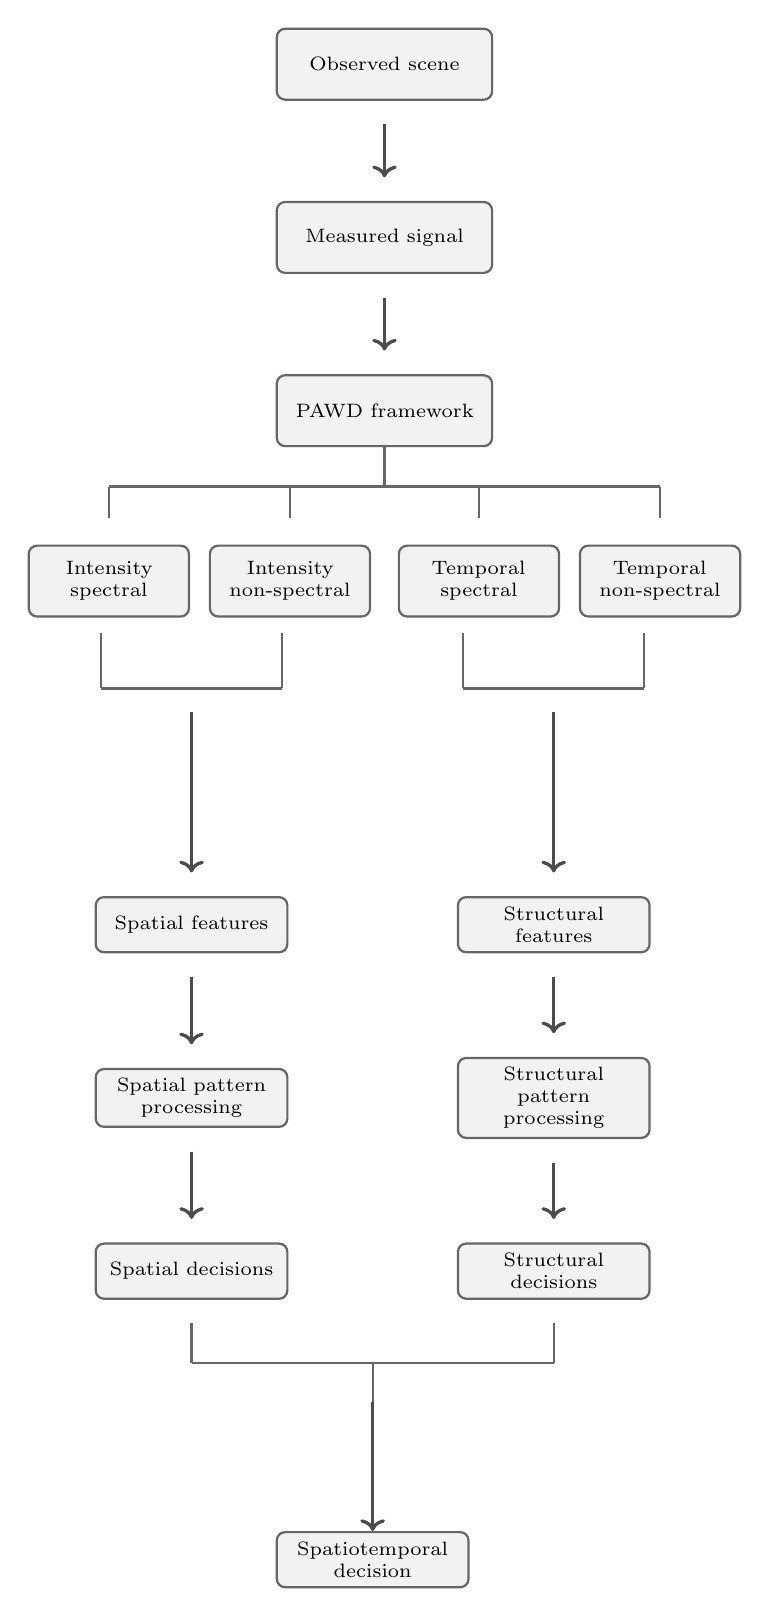
\begin{tikzpicture}[
    node distance=2.2cm, 
    auto,
    every node/.style={font=\scriptsize},
    main node/.style={rectangle, draw=black!60, fill=gray!10, text width=2.5cm, align=center, minimum height=0.9cm, rounded corners=3pt, line width=0.8pt, font=\scriptsize},
    item node/.style={rectangle, draw=black!60, fill=gray!10, text width=1.8cm, align=center, minimum height=0.9cm, rounded corners=3pt, line width=0.8pt, font=\scriptsize},
    process node/.style={rectangle, draw=black!60, fill=gray!10, text width=2.2cm, align=center, minimum height=0.7cm, rounded corners=3pt, line width=0.8pt, font=\scriptsize}
]
    % Define nodes vertically
    \node[main node] (scene) {Observed scene};
    \node[main node, below of=scene] (signal) {Measured signal};
    \node[main node, below of=signal] (pawd) {PAWD framework};
    
    % Draw arrows vertically with gaps (not touching boxes)
    \draw[->, line width=1.2pt, color=black!70] ([yshift=-0.3cm]scene.south) -- ([yshift=0.3cm]signal.north);
    \draw[->, line width=1.2pt, color=black!70] ([yshift=-0.3cm]signal.south) -- ([yshift=0.3cm]pawd.north);
    
    % Short vertical line from PAWD framework
    \draw[line width=0.8pt, color=black!60] (pawd.south) -- ++(0,-0.5cm) coordinate (pawd_bottom);
    
    % Horizontal line spanning 4 items
    \draw[line width=0.8pt, color=black!60] ([xshift=-3.5cm, yshift=0cm]pawd_bottom) -- ([xshift=3.5cm, yshift=0cm]pawd_bottom);
    
    % Four items arranged horizontally
    \node[item node, below of=pawd_bottom, xshift=-3.5cm, yshift=1.0cm] (item1) {Intensity\\spectral};
    \node[item node, below of=pawd_bottom, xshift=-1.2cm, yshift=1.0cm] (item2) {Intensity\\non-spectral};
    \node[item node, below of=pawd_bottom, xshift=1.2cm, yshift=1.0cm] (item3) {Temporal\\spectral};
    \node[item node, below of=pawd_bottom, xshift=3.5cm, yshift=1.0cm] (item4) {Temporal\\non-spectral};
    
    % Short vertical lines from horizontal line to each item
    \draw[line width=0.8pt, color=black!60] ([xshift=-3.5cm, yshift=0cm]pawd_bottom) -- ++(0,-0.4cm);
    \draw[line width=0.8pt, color=black!60] ([xshift=-1.2cm, yshift=0cm]pawd_bottom) -- ++(0,-0.4cm);
    \draw[line width=0.8pt, color=black!60] ([xshift=1.2cm, yshift=0cm]pawd_bottom) -- ++(0,-0.4cm);
    \draw[line width=0.8pt, color=black!60] ([xshift=3.5cm, yshift=0cm]pawd_bottom) -- ++(0,-0.4cm);
    
    % Second horizontal line below the 4 items
    \coordinate (items_bottom) at ([yshift=-1.0cm]item2.south);
    
    % Four vertical lines pointing upward
    \draw[line width=0.8pt, color=black!60] ([xshift=-2.4cm, yshift=0.8cm]items_bottom) -- ++(0,-0.7cm);
    \draw[line width=0.8pt, color=black!60] ([xshift=-0.1cm, yshift=0.8cm]items_bottom) -- ++(0,-0.7cm);
    \draw[line width=0.8pt, color=black!60] ([xshift=2.2cm, yshift=0.8cm]items_bottom) -- ++(0,-0.7cm);
    \draw[line width=0.8pt, color=black!60] ([xshift=4.5cm, yshift=0.8cm]items_bottom) -- ++(0,-0.7cm);
    
    % Horizontal lines below items (just below the bottom vertical lines)
    % First horizontal line connecting the first 2 bottom vertical lines
    \draw[line width=0.8pt, color=black!60] ([xshift=-2.4cm, yshift=0.1cm]items_bottom) -- ([xshift=-0.1cm, yshift=0.1cm]items_bottom);
    % Second horizontal line connecting the 3rd and 4th bottom vertical lines
    \draw[line width=0.8pt, color=black!60] ([xshift=2.2cm, yshift=0.1cm]items_bottom) -- ([xshift=4.5cm, yshift=0.1cm]items_bottom);
    
    % Items under first bottom horizontal line (spatial)
    \node[process node, below of=items_bottom, xshift=-1.25cm, yshift=-0.7cm] (spatial_features) {Spatial features};
    \node[process node, below of=spatial_features] (spatial_pattern) {Spatial pattern\\processing};
    \node[process node, below of=spatial_pattern] (spatial_decisions) {Spatial decisions};
    
    % Arrow from horizontal line to spatial features (matching gap between items)
    \draw[->, line width=1.2pt, color=black!70] ([xshift=-1.25cm, yshift=-0.2cm]items_bottom) -- ([yshift=0.3cm]spatial_features.north);
    % Arrows for spatial flow
    \draw[->, line width=1.2pt, color=black!70] ([yshift=-0.3cm]spatial_features.south) -- ([yshift=0.3cm]spatial_pattern.north);
    \draw[->, line width=1.2pt, color=black!70] ([yshift=-0.3cm]spatial_pattern.south) -- ([yshift=0.3cm]spatial_decisions.north);
    
    % Items under second bottom horizontal line (structural)
    \node[process node, below of=items_bottom, xshift=3.35cm, yshift=-0.7cm] (structural_features) {Structural features};
    \node[process node, below of=structural_features] (structural_pattern) {Structural pattern\\processing};
    \node[process node, below of=structural_pattern] (structural_decisions) {Structural decisions};
    
    % Arrow from horizontal line to structural features (matching gap between items)
    \draw[->, line width=1.2pt, color=black!70] ([xshift=3.35cm, yshift=-0.2cm]items_bottom) -- ([yshift=0.3cm]structural_features.north);
    % Arrows for structural flow
    \draw[->, line width=1.2pt, color=black!70] ([yshift=-0.3cm]structural_features.south) -- ([yshift=0.3cm]structural_pattern.north);
    \draw[->, line width=1.2pt, color=black!70] ([yshift=-0.3cm]structural_pattern.south) -- ([yshift=0.3cm]structural_decisions.north);
    
    % Connect the last two items (spatial decisions and structural decisions)
    % Two vertical lines going up from each decision box
    \draw[line width=0.8pt, color=black!60] ([yshift=-0.3cm]spatial_decisions.south) -- ++(0,-0.5cm) coordinate (spatial_decisions_bottom);
    \draw[line width=0.8pt, color=black!60] ([yshift=-0.3cm]structural_decisions.south) -- ++(0,-0.5cm) coordinate (structural_decisions_bottom);
    
    % Horizontal line connecting the two vertical lines
    \draw[line width=0.8pt, color=black!60] (spatial_decisions_bottom) -- (structural_decisions_bottom);
    
    % Vertical line from centre of horizontal line (single continuous line, 0.5cm like first vertical line)
    % Create coordinate at midpoint: spatial at x=-1.25cm, structural at x=3.35cm, midpoint at x=1.05cm
    \path (spatial_decisions_bottom) -- (structural_decisions_bottom) coordinate[midway] (horizontal_mid);
    \draw[line width=0.8pt, color=black!60] (horizontal_mid) -- ++(0,-0.5cm) coordinate (spatiotemporal_top);
    
    % Spatiotemporal decision item (positioned below the vertical line)
    \node[process node, below of=spatiotemporal_top, yshift=0.2cm] (spatiotemporal_decision) {Spatiotemporal decision};
    
    % Arrow from vertical line to spatiotemporal decision (single continuous arrow)
    \draw[->, line width=1.2pt, color=black!70] (spatiotemporal_top) -- (spatiotemporal_decision.north);
\end{tikzpicture}
}
\caption[Flow chart showing the processing pipeline from observed scene through measured signal to the PAWD framework.]{Flow chart showing the processing pipeline from observed scene through measured signal to the PAWD framework. Intensity measured signal is often spatially resolved to represent scenes. Nevertheless, time resolved signal may also be spatially resolved. This is termed space resolved temporal measurements (SRTM). SRTM are not useful for structural decisions. However, they may play key roles in spatial decisions like pose estimation, scale estimation and others. A true spatiotemporal solution is one that combines the crude time resolved signal with intensity resolved signal for decision making.}
\label{fig:1_1}
\end{figure}

\textbf{Figure 2:} Signal processing flow diagram illustrating temporal and spatial signal paths

\textbf{Figure 3:} Material detection module architecture (16$\times$16$\times$3 input, convolutional layers, classification head)

\textbf{Figure 4:} Example detection results showing object localisation with material classification

\vspace{0.5em}
\subsection{DECLARATION}

We, A. Akuoko, D. Chitnis, and I. Gyongy, declare that:
1. We are the inventors of the invention described in this application;
2. The invention has not been publicly disclosed prior to the filing date of this application;
3. To the best of our knowledge, the invention is novel and involves an inventive step;
4. We are entitled to apply for a patent for this invention.

\textbf{Signature:} _________________________

\textbf{Date:} _________________________

\vspace{0.5em}
\textbf{END OF SPECIFICATION}

\end{enumerate}

\end{document}
